\subsection{Roulette Selection}
El mecanismo de selección de ruleta, es una técnica popularmente usada en algoritmos genéticos para seleccionar posibles soluciones de acuerdo a su aptitud. La idea es dar a cada individuo una probabilidad de ser seleccionado que sea proporcional a su aptitud, de tal manera que los individuos con mayor aptitud tengan una mayor probabilidad de ser elegidos, pero aún permitiendo que los individuos con menor aptitud tengan alguna posibilidad.

En términos generales, este método consta de los siguientes pasos:

\begin{enumerate}
	\item Cálculo de Aptitudes: En primer lugar, se calcula la aptitud de cada individuo en la población.
	\item Suma de Aptitudes: Se suman todas las aptitudes para obtener una aptitud total de la población.
	\item Cálculo de Probabilidades: Se determina la probabilidad de selección de cada individuo dividiendo su aptitud por la aptitud total de la población.
	\item Selección: Se genera un número aleatorio entre 0 y 1. Luego, se selecciona el individuo cuya probabilidad acumulada incluye este número aleatorio. En otras palabras, imaginamos que giramos una ruleta donde cada segmento corresponde a un individuo, y el tamaño de cada segmento es proporcional a la aptitud del individuo.
\end{enumerate}

Una representación gráfica de este mecanismo se puede observar en la Figura \ref{fig:RS}.

\begin{figure}[htbp]
	\centering
	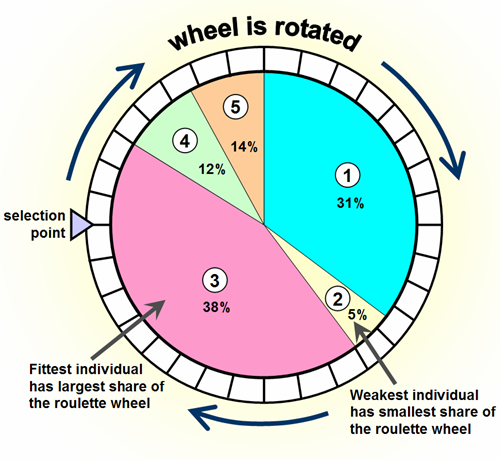
\includegraphics[width=0.4\textwidth]{roulette_selection}
	\caption{Diagrama de funcionamiento de selección por ruleta.}
	\label{fig:RS}
\end{figure}


\subsection{Tournament Selection}
El mecanismo de selección por torneo es otro método popular utilizado en algoritmos genéticos para seleccionar individuos de una población basándose en su aptitud. Es un método relativamente simple y eficiente que puede adaptarse fácilmente para dar preferencia a individuos con mayor o menor aptitud.

La aproximación seleccionada para este trabajo consiste en realizar parejas de adentro hacia afuera dentro del conjunto de individuos. Esta aproximación presenta un problema en poblaciones grandes, ya que la diferencia de aptitud entre el individuo más alto y el menos apto es grande.

Este mecanismo se puede representar gráficamente mediante la Figura \ref{fig:TS}.

\begin{figure}[htbp]
	\centering
	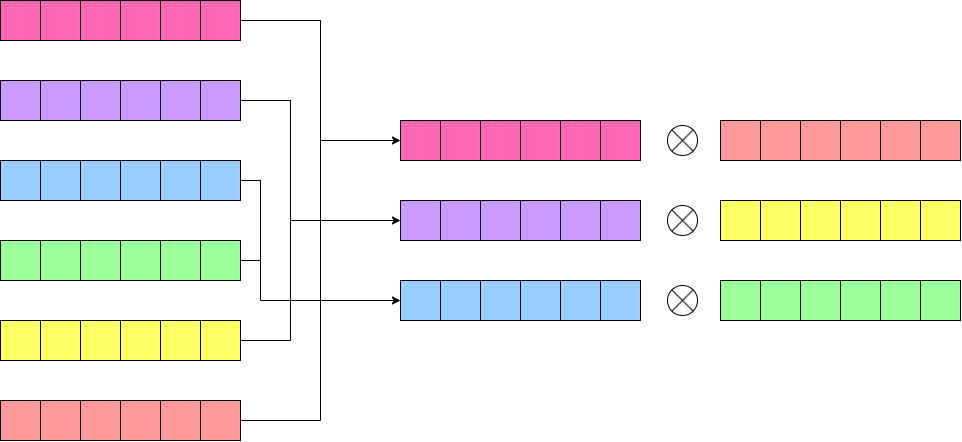
\includegraphics[width=0.8\textwidth]{tournament_selection}
	\caption{Diagrama de funcionamiento de selección por torneo.}
	\label{fig:TS}
\end{figure}


\subsection{Partially Mapped Crossover}
El Partially Mapped Crossover (PMx) es una técnica de cruce especialmente diseñada para problemas de optimización combinatoria en los que las soluciones son representaciones de permutaciones de números. El objetivo del PMx es transferir sin ambigüedades segmentos de información entre dos padres, garantizando que los hijos resultantes sean permutaciones válidas.

El algoritmo consta de la siguiente serie de pasos:

\begin{enumerate}
	\item Selección de un Segmento: Se seleccionan aleatoriamente dos puntos de corte en los padres, que definen un segmento.1
	\item Intercambio de Segmentos: Se intercambian los segmentos entre los dos padres para formar la base de los dos hijos.
	\item Reemplazo Fuera del Segmento: Para cada posición fuera del segmento intercambiado:
	\begin{enumerate}
		\item Si el número en la posición correspondiente del otro padre ya está presente en el segmento intercambiado, se busca el número que ocupa esa posición en el segmento original y se sigue rastreando las posiciones hasta encontrar un número que no esté en el segmento intercambiado.
		\item Se reemplaza el número en la posición actual del hijo con el número encontrado en el paso anterior.
	\end{enumerate}
	\item Finalización: Se repite el paso anterior hasta que todos los números fuera del segmento intercambiado en ambos hijos son permutaciones válidas de los números originales.
\end{enumerate}

Este mecanismo se puede representar gráficamente como se muestra en la Figura \ref{fig:PMx}.

\begin{figure}[htbp]
	\centering
	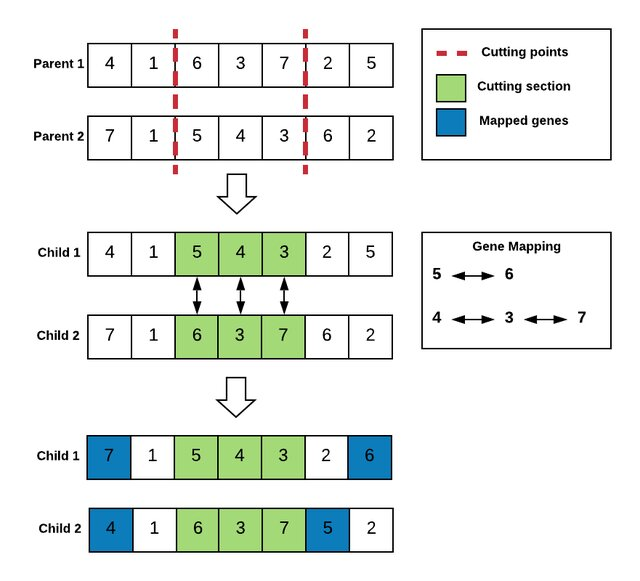
\includegraphics[width=0.7\textwidth]{pmx}
	\caption{Diagrama de funcionamiento de partially mapped crossover.}
	\label{fig:PMx}
\end{figure}


\newpage
\subsection{Cycle Crossover}
El Cycle Crossover (Cx) es otro operador de cruce específico para representaciones de permutación en algoritmos genéticos. A diferencia del PMx, el Cx se centra en la preservación de la posición absoluta de cada alelo, lo que puede conducir a una transmisión más consistente de ciertos rasgos de los padres a los hijos.

Los pasos generales de dicho mecanismo son:
\begin{enumerate}
	\item Inicio del Primer Ciclo: Comienza con el primer elemento del primer padre.
	\item Formación de Ciclos:
	\begin{enumerate}
		\item Mira la posición de ese elemento en el segundo padre.
		\item Ve al elemento del primer padre en esa misma posición.
		\item Repite este proceso hasta que regrese al elemento inicial del primer padre. Ahora, tienes un ciclo.
	\end{enumerate}
	\item Transferencia de Ciclos a los Hijos:
	\begin{enumerate}
		\item Transfiere todos los elementos del primer ciclo del primer padre al primer hijo en las mismas posiciones. Haz lo mismo para el segundo hijo pero usando los alelos del segundo padre.
	\end{enumerate}
	\item Formación de Ciclos Adicionales:
	\begin{enumerate}
		\item Si aún quedan elementos sin asignar en los hijos, repite el proceso de formación de ciclos comenzando desde el primer elemento no asignado en el primer padre y crea otro ciclo.
		\item Alterna entre los padres para determinar qué alelos se transfieren a los hijos para cada ciclo adicional.
	\end{enumerate}
	\item Finalización: Continúa hasta que todos los elementos están asignados en ambos hijos.
\end{enumerate}

Este mecanismo se puede representar graficamente como se muestra en la Figura \ref{fig:Cx}.

\begin{figure}[htbp]
	\centering
	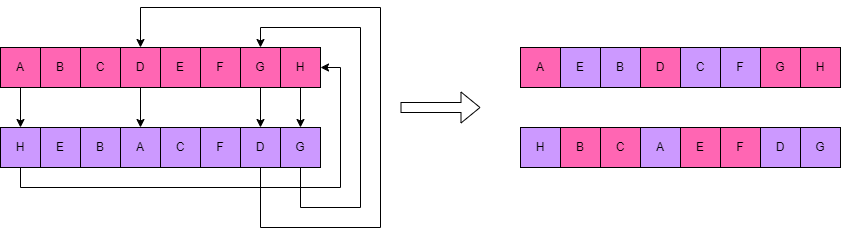
\includegraphics[width=0.8\textwidth]{cx}
	\caption{Diagrama de funcionamiento de cycle crossover.}
	\label{fig:Cx}
\end{figure}


\FloatBarrier
\subsection{Insert Mutation}
El proceso Insert Mutation, es una técnica de mutación utilizada en algoritmos genéticos para modificar soluciones que se representan como permutaciones. Es especialmente útil en problemas donde las soluciones son representaciones de rutas o secuencias.

Los pasos de este proceso son:
\begin{enumerate}
	\item Selección de segmentos: Se seleccionan aleatoriamente dos segmentos en la permutación, asegurándose de que no sean el misma segmento.
	\item Inserción: Se intercambian los segmentos entre ellos.
\end{enumerate}

Este mecanismo se puede observar en la Figura \ref{fig:IsrM}

\begin{figure}[htbp]
	\centering
	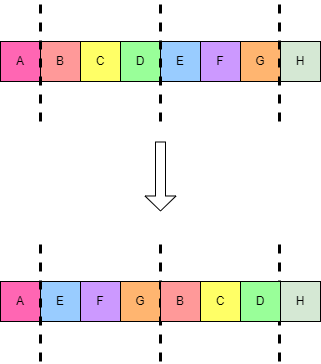
\includegraphics[width=0.4\textwidth]{insert_mutation}
	\caption{Diagrama de funcionamiento de insert mutation.}
	\label{fig:IsrM}
\end{figure}


\subsection{Inverse Mutation}
La mutación por inversión, o "Inverse Mutation", es otra técnica de mutación usada en algoritmos genéticos que trabajan con soluciones representadas como permutaciones. El procedimiento de esta técnica consta de los siguientes pasos:

\begin{enumerate}
	\item Selección de segmento: Se seleccionan aleatoriamente dos puntos en la permutación. Estos puntos determinarán el inicio y el fin de un segmento.
	\item Inversión: El segmento delimitado por estos dos puntos se invierte, es decir, el orden de los alelos dentro de este segmento se revierte.
\end{enumerate}

Este mecanismo se puede observar en la Figura \ref{fig:InvM}

\begin{figure}[htbp]
	\centering
	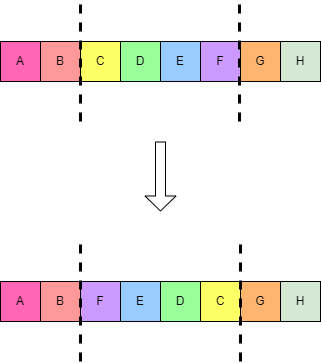
\includegraphics[width=0.4\textwidth]{inverse_mutation}
	\caption{Diagrama de funcionamiento de inverse mutation.}
	\label{fig:InvM}
\end{figure}
